% Candidate source: src-22a421a422f050bc84accae7bf41feb6903c62df04bd83f34d8267d28f49ee2e
% Source PDF SHA-256: 092e8e90dc1430ab2fa8b8ce79e072e317559e6bef29f1cb7461e9423925ec31
% PDF page 1 (printed page 262), question 19.
% Redraw follows visible relations; point placement is schematic, not a scale claim.
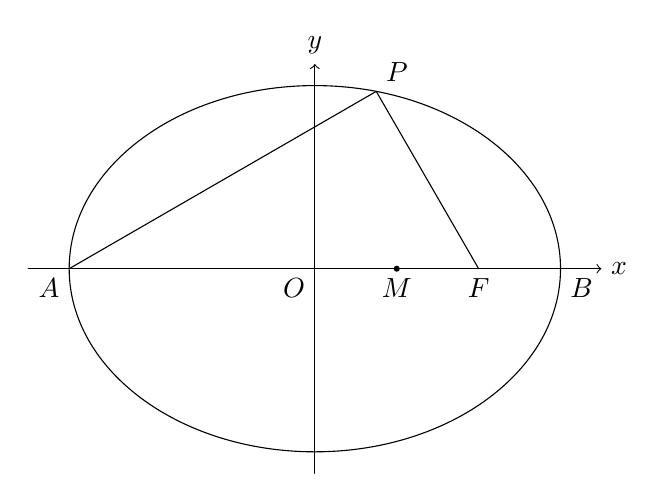
\begin{tikzpicture}[line cap=round,line join=round,x=0.52cm,y=0.52cm]
  \coordinate (A) at (-6,0);
  \coordinate (B) at (6,0);
  \coordinate (F) at (4,0);
  \coordinate (M) at (2,0);
  \coordinate (P) at (1.5,{5*sqrt(3)/2});

  % Ellipse and coordinate axes.
  \draw (0,0) ellipse [x radius=6,y radius={sqrt(20)}];
  \draw[->] (-7,0)--(7,0) node[right] {$x$};
  \draw[->] (0,-5)--(0,5) node[above] {$y$};

  % Chords shown in the source figure.
  \draw (A)--(P)--(F);
  \fill (M) circle (1.1pt);

  \node[below left] at (A) {$A$};
  \node[below right] at (B) {$B$};
  \node[below left] at (0,0) {$O$};
  \node[below] at (M) {$M$};
  \node[below] at (F) {$F$};
  \node[above right] at (P) {$P$};
\end{tikzpicture}
